\let\textcircled=\pgftextcircled


\chapter{Literature Review}
\label{chap:lit_review}

The idea of autonomous vehicles(AVs) is not new. As early as 2005, DARPA had invested heavily in the creation of unmanned trucks and organised for the Urban Challenge \cite{buehler2009darpa} to allow for different teams to showcase their unmanned vehicles. However, due to the challenges such as low computational power and underdeveloped AI and ML systems, the resulting implementations were not practical and had a high fault rate of 1 fault in 100 miles compared to the human fault rate of around 1 in 100 million miles. Nonetheless, from this challenge, it was clear that the prospect of AVs was plausible and indeed possible. 

Currently, AVs are divided into five levels as defined by the National Highway Traffic Safety Administration(NHTSA) depending on their level of autonomy. 
\begin{itemize}
	\item \textbf{Level 0} - No autonomy. 
	\item \textbf{Level 1} - Basic driver assistance built into vehicle design.
	\item \textbf{Level 2} - Partially autonomous but driver expected to monitor environment at all times.
	\item \textbf{Level 3} - Conditionally autonomous with the driver not required to monitor the environment but is required to take back control if need be.
	\item \textbf{Level 4} - Highly autonomous with the vehicle capable of handling most conditions but the driver has the option to take control. 
	\item \textbf{level 5} - Completely autonomous with the vehicle capable of handling all conditions.
\end{itemize}

The race to level 5 autonomous by different companies has seen major competition between these industry players. As such, they have invested heavily in designing and deploying AVs. However, these vehicles tend to have various sensors as seen in figure \ref{fig:my_label}. These sensors are necessary for accurate navigation and safety. Nonetheless, they are quite expensive thereby making AVs not feasible at the moment. 
\section{Components of an AV}

Most self-driving cars consist of 4 main components: 
\begin{itemize}
	\item \textbf{LiDAR} - LiDAR provides highly detailed 3D information about the environment around the vehicle and objects in it. LiDAR operates by sending out pulses of lasers and recording the reflections of the pulses from objects. By comparing this with the time taken for the lasers to be reflected(time of flight) and their direction, the distance of these objects can be calculated and mapped in a point cloud. 

	LiDAR units require complex optical systems that are expensive to build. As a result,  they are the most expensive sensors in AVs with the top end such as Velodyne HDL-64E shown in figure \ref{fig:lidar} costing more than 50,000\$. 
	In a bid to reduce the cost of LiDAR units,  different companies are exploring different design methods that are cheaper but still able to offer the same performance as the top end LiDAR units such as solid state LiDAR\footnote{See appendix \ref{app:lidar}}.
	
	 \begin{figure}[h]
	 	\centering
	 	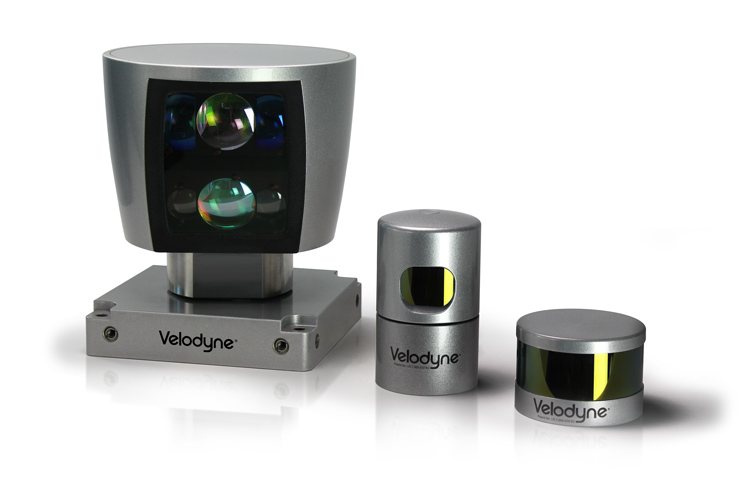
\includegraphics[width=\textwidth]{media/hdl-family.png}
	 	\caption{Velodyne LiDAR family. From left: Velodyne HDL-64E , HDL-32E , PUCK}
	 	\label{fig:lidar}
	 \end{figure}
	
	\item \textbf{Cameras} - Cameras mounted on the vehicle are used for classification and identification of various objects on the road. 
	Cameras can also be used to create 3D maps of the surrounding environment.By combining two cameras, a stereo image can be captured that provides depth information. Alternatively, by combining a camera and IR Laser sensor for depth estimation, RGB-D \cite{henry2010rgb} images are obtained and mapped in a point cloud.
	
	\item \textbf{Position Estimators} - Position estimators are a group of sensors used for navigation of the vehicle. These include GPS systems, odometers and gryometers. 
	\item \textbf{Distance Sensors} - Distance sensors such as radars and sonars are important for gauging the distance of objects on the road. 
	Radars are the most commonly used distance sensors and they work by transmitting radio waves and recording the reflected radio waves from objects. As compared to cameras and LiDARs, radars work well in a variety of low visibility scenarios such as poor weather. 
	However, the reflectivity of these radio waves depends on the nature of objects, their size, absorbtion characteristics and the transmitting power. As such, it is may not be effective for detecting objects with low absorbtion characteristics such as pedestrians and animals.
	
	\item \textbf{Processing Unit} - In order to process all the data from sensors on the vehicle, AVs require powerful processing units to to do so in real time. Most ML/AI algorithms used for detecting and identifying objects from LiDAR and camera data demand large amounts of processing power. This is achieved through the use of CPUs, GPUs, Field Programmable Gate Arrays(FPGA)\cite{brown2012field}, Application Specific Integrated Circuits(ASICs)\cite{smith1997application} or combinations with each other. 

\end{itemize}


\begin{figure}[t]
	\centering
	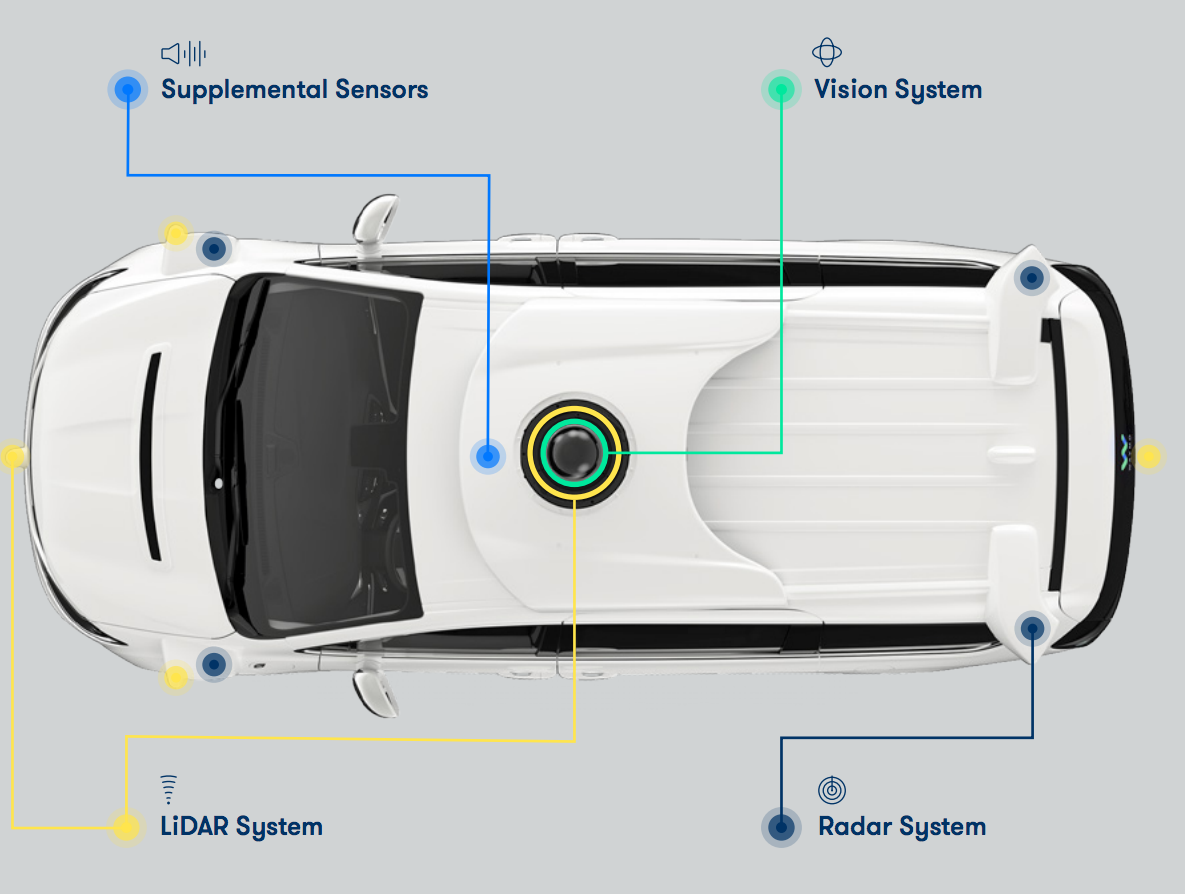
\includegraphics[width=\textwidth]{media/waymo.png}
	\caption{Components of Waymo's Self Driving Car \cite{waymo_2018}}
	\label{fig:my_label}
\end{figure}



\section{Legal, Ethical and Economic Considerations}

The classic ethical dilemma for self driving cars poses a scenario whereby AVs are presented with a situation whereby a fatal accident is inevitable. For example, the AV either has to crash into a group of people in order to save the life of a passenger or to crash itself and sacrifice the life of the passenger. This dilemma highlights important legal, ethical and economic considerations to be considered by companies involved in the production of AVs and their corresponding systems. 


According to \cite{gasser2016fundamental}, there are no public laws that cover the  use of independent autonomous vehicles in public spaces. In his article, he cites the fundamental issue as "understanding and accepting the effect of AVs as an independent action by a machine". Due to the lack of public laws on their use, he proposes extending fundamental rights such as the right to life into the framework for creating laws that cover emerging technologies that have an effect on the public, that are otherwise not accounted for in traditional laws. 

Bearing this in mind, it is important to note that despite improvements in traffic safety over the years, 94\% are still caused by human beings with a large majority of them being fatal with the current human error rate being 1 in 100 million miles. This creates a realistic baseline that can then be extended in evaluating the performance of AV systems. As such, if the risk of automation is lesser than the risk of human vehicle control then the AV would be beneficial. Consequently, the AVs are not to be considered as perfect systems.

With regard to economic considerations, car manufacturers involved in the production of AVs have to ensure that their AVs are able to handle numerous scenarios even if they are rare or considered statistically impossible. They should also be required to take legal liability in case any of their system components are defective and result in failures or accidents. This is important for customer trust without which they will not be able to convince customers to shift to AVs. In addition, for the adoption of AVs to be widespread, they have to be reasonably priced and efficient. With the current prices of the the various components and their power consumption, the adoption of AVs at the moment is not viable. 



AVs have three main modes of operation namely,
\begin{itemize}
	\item \textbf{Perception} - This is the first step which involves processing the input from the sensors. In this mode tasks such as object detection and tracking, lane detection, traffic sign detection and recognition are performed.
	\item \textbf{Planning} - This is the next step after detection and recognition tasks are performed . In this stage route and trajectory planning algorithms are run  to plan how the vehicle should navigate in the immediate environment as well as a route to a target location. These algorithms are required to handle complex situations to ensure safety of the passengers and other road users. 
	\item \textbf{Control} - This stage involves the execution of plans created in the planning stage. This stage is crucial as the actuators involved in steering and movement have to be able to be able to accurately follow the plans. This involves calculation of energy and forces. At this stage the trajectories and movement of other road users and objects have to be calculated in order to anticipate and avoid any accidents. 
	
\end{itemize}



\section{Industrial Approaches}
In order to be viable, AVs need to meet a few constraints as discussed in \cite{lin2018architectural}.
\begin{itemize}
	\item \textbf{Performance} \\
	At the moment there are no clear regulations as to how fast the perception, planning and control pipeline should be. However according to research by Brown et al. \cite{brown1994human}, humans take around 600 ms to respond and brake when expecting an interruption, however this figure shoots to 850 ms when an unexpected situation arises. In addition, Newell et al \cite{newell1985prospects}, established that the fastest human response time is between 100-150ms. These figures can be used as a baseline while developing a pipeline. In this pipeline, there are two factors to consider, namely the frame rate (frequency of the data from sensors) and the processing latency (time taken to process data). As such, an AV system should be able to react within 100ms, that is, faster than the human response time.
	
	\item \textbf{Storage} \\ 
	AVs should be able to store maps of different areas with fine granularity for accuracy during localisation. As a result, the storage of these maps can run into tens of Terabytes. Despite recent advances in cloud technology and the emergence of 5G connectivity that is significantly fast. Downloading these maps would take significant time and would also render the car unusable in case of no internet connectivity. As such, the vehicles should have enough storage to store these maps locally. 
	
	\item \textbf{Power} \\
	Most of the major industry players have moved to electric-vehicles for their AV systems. Depending on the equipment and sensor configurations used in these systems, the power usage can range from 500 watts to 1.5 kilowatts. Given that the AVs have limited battery capacity, heavy power consumption by these systems can lead to poor driving ranges hence making the cars less viable. As such the configuration of these systems has to be carefully considered to ensure a reasonable driving range. 

	\item \textbf{Thermal} \\
	Processing components in the AV systems such as CPUs and GPUs require a significant amount of energy to cool. This is necessary to ensure that they operate within their recommended thermal operating range. Failure to do so could result in the failure of these systems. As such, additional cooling systems have to be installed in the vehicle in order to ensure this.
	
\end{itemize}
Following the discussion above, the next subsections will review how different industry players are implementing their AV systems with special focus to the issue of perception
\begin{figure}
	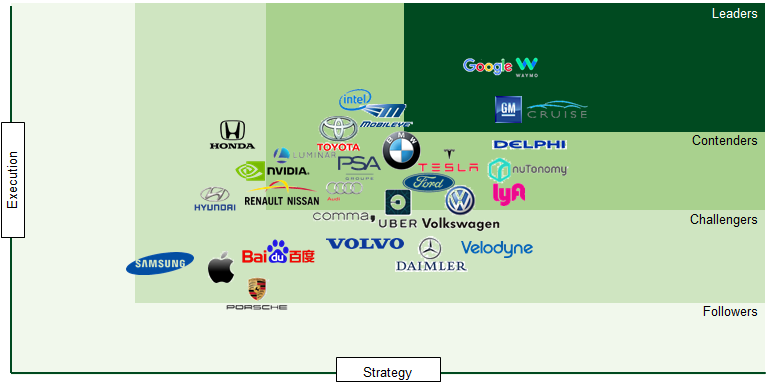
\includegraphics[width=\textwidth]{media/avind.png}
	\caption{AV Leaderboard. Navigant Research\cite{navigantresearch_2018}}
\end{figure}
\subsection{Camera}
Mobileye\cite{mobileye_2018}, is one of the top contenders in the development of camera only AVs. It was recently acquired by Intel and believes that AVs should be able to accurately and safely navigate using cameras only given the fact that humans are able to do so with vision only. Previously, MobilEye was a supplier of vision systems for Advanced Driver Assistance Systems and had a partnership with Tesla to supply their vision systems prior being acquired by Intel. 
Given their extensive background in developing these vision systems, the partnership with Intel aims to develop a complete autonomous driving package.\cite{intelsolutions_2018}
 

\subsection{Camera and  Radar}
Another major contender that is using the camera and radar configuration is Tesla. Elon Musk, the founder, believes that LiDAR is not necessary for AV perception. However, just recently, a Tesla vehicle was involved in a crash while in 'autopilot' mode that resulted in the loss of life. A major attributing factor to this accident was caused by the fact that bright sunlight blinded the camera thus causing the vehicle not to detect a white truck that was ahead of it. The radar was also unable to detect it thus leading to a collision. 
LiDAR on the other hand, would have been able to detect the truck despite the poor visibility. This illustrates how unreliable this configuration can be.


\subsection{LiDAR, Camera and Radar}
This configuration is used by most of the leading industry players such as Waymo and GM Cruise. This configuration has proven to be robust and accurate.
 However, in order to process the amount of fused data, they require large amounts of processing power which in turn may lead to increased power usage. In addition due to the number of sensors, the cost of these AVs is quite high and therefore not economically feasible. 


\section{Related Research} 
\subsection{Classic Computer Vision}
With regard to perception, classic computer vision methods have advanced over the years from simple algorithms such as SIFT\cite{lowe1999object} and SURF\cite{bay2006surf} which use descriptors to detect interesting points in images for object detection to much higher level representations such as the Histogram of Gradient(HOG)\cite{dalal2005histograms} or Haar Features\cite{viola2001rapid}  that were used in classifiers.  However, these methods have been unreliably slow and not as accurate. In addition these features are only able to model 2D data and therefore when applied to 3D data such as point clouds they are unusable. Furthermore, these feature detectors have to be hand-crafted manually which is a tedious process. As a result,  such classical methods can not be used in AVs as they are not as robust and accurate.  


\subsection{Deep Neural Networks}

The emergence and development of Deep Neural Networks such as Convolutional Neural Networks (CNNs)\cite{lawrence1997face} has offset the reliance of classical methods of object detection in images by allowing for features to be automatically learnt by the network without the need for manual feature extraction. This is due to the fact that these networks have numerous number of deep layers that are able to capture these features.  

\textbf{Monocular and Stereo Vision} \\ 
Due to the high prices of LiDAR units, there were many attempts to develop detection methods that would use standard cameras that were cheap and readily available.
Chen et al \cite{chen2016monocular} of Baidu Inc. developed a 3D proposal method from monocular images that would then be used as input to CNNs. In this method, 2D objects were detected in the images and then extruded into 3D using  class segmentation, instance level segmentation, shape,
contextual features and location priors. This method was one of the best performing monocular object detection  method according to the KITTI Benchmark. However, this method only performed well in well lit environments. It's performance declined greatly in dark scenes. In addition, due to the lack of depth information, the accuracy of the method is entirely dependent on the segmentation of detected 2D objects. Furthermore, the source code of this paper was never released thus making it difficult to validate the results with other datasets

Another attempt at developing lower cost detection systems was through the use of stereo cameras. This involved deploying and calibrating two cameras and through stereo matching and reprojection, a 3D image could be obtained that contains depth information. However as with monocular systems, they suffered the same issue of poor performance in dark scenes. In light of this, such methods would not be viable for use in AVs. 



\textbf{Multimodal } \\
In an effort to improve the accuracy and robustness of AVs, multimodal methods were developed. This involves combining both LiDAR and camera or a camera and a range finder(RGB-D). Both these configurations provide depth information in the form of point clouds. 
Chen et al further reiterated their monocular approach into MV3D\cite{chen2017multi} a multiview 3D object detection network. In their work, they were able to fuse LiDAR and camera input to create a bird's eye view of the surrounding environment and further perform object detection of features. Similarly as before, the source code was never released and therefore their results cannot be validated with other datasets. 


\textbf{LiDAR} \\ 
Point cloud object detection is particularly challenging as established 3D object detection methods for images cannot be applied to point clouds. Point clouds are a set of geometric points in a euclidean space. They are unordered in nature and this presents a particular problem to DNNs as they need to be invariant to permutations of the input set.

Pointnet\cite{qi2017pointnet} developed by Qi et al was able to overcome this challenge on small sets of point clouds. By using point clouds as direct input into Recurrent Neural Networks\cite{medsker2001recurrent} They were able to create a global point cloud signature that could classify and segment 3D objects in the point cloud. They further improved this model into Pointnet++\cite{qi2017pointnet++} which recursively applied PointNet on nested partitions of the point clouds using a hierarchical neural network. In doing so they were able to capture the local structures of the point clouds as a result of their metric nature and thus achieve better performance than PointNet. For both of these publications, the source code was released for public use. Consequently, they have formed a fundamental foundation for further development of point cloud object detection methods.

An attempt at detecting objects in point clouds from a  LiDAR mounted in a vehicle was performed by \cite{li20163d}. In their work, they used a Fully Convolutional Network (FCN) to detect and localise objects in a point cloud as 3D bounding boxes. They were able to achieve this by discretising the point clouds into square grids represented by a 4D array containing the dimensions and a channel indicating if there was a point at that space in the grid. It performed significantly well in the KITTI benchmark. However, the source code was not released. 

Finally, \cite{zhou2017voxelnet}  were able to create a point cloud based 3D object detection network by adding a Voxel Feature Extraction layer before a RPN that was able to divide the point cloud into voxels that were used as input for the RPN. The published results were well above the state of the art LiDAR object detection methods. As is the case with other publications, the source code was not released and therefore cannot be validated.  

\section{Deep Learning Framework}

 As mentioned in the previous chapter one of the main deliverables will be an end to end RPN model for detecting objects in point clouds. In order to develop this I will make use of a deep learning framework. 
At the moment, there are various distributions of deep learning frameworks that are available for different programming languages. 
A few popular ones include:
\begin{table}[H]
	\centering
	\begin{tabular}{|c|c|}
		\hline
		Framework & Programming Language(s)  \\ \hline
		Tensorflow &  Python, C++ , R  \\ \hline
		PyTorch & Python  \\ \hline
		Caffe & C, C++, Python, MATLAB \\ \hline
		MXNet & Python, C++, R, Julia \\ \hline
		Microsoft Cognitive Toolkit/CNTK & Python, C++ \\ \hline
		
	\end{tabular}
	\caption{Popular deep learning frameworks}
	\label{table:dlframeworks}
\end{table}

\subsection{TensorFlow CNN}
I intend to use Tensorflow on Python to implement the RPN for the following reasons.
\begin{enumerate}
	\item \textbf{Large support community }
	\item \textbf{Quick prototypying}
	\item \textbf{Well tested and reliable}
	\item \textbf{Portable}
\end{enumerate}
Figure \ref{ fig:cnn_vis} illustrates a simple CNN visualisation which forms a major part of the RPN model.  A python implementation  can be found in Appendix \ref{app:app01}

\begin{figure}[h]
	\centering
	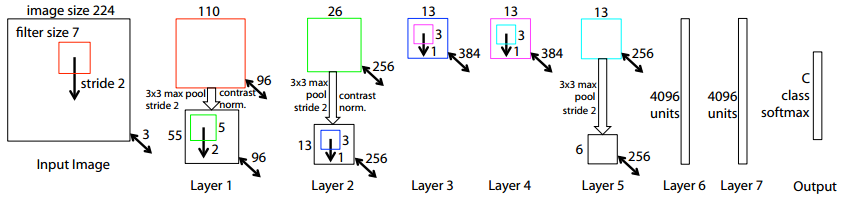
\includegraphics[width=\textwidth]{media/cnn.png}
	\caption{CNN Visualisation \cite{zeiler2014visualizing}}
	\label{ fig:cnn_vis}
\end{figure}






